\subsection{Rundkørsel}
\label{sub:rundkoersel}
En løsningsforslag kan være rundkørsel. Ved blot at kigge på rundkørsel, så kan der hurtig ses, at farten vil blive sænket ved de områder hvor der er rundkørsel. Får man indført rundkørsel ved Nytorv området, så vil hypotesen være at cyklister pr. automatik sænker farten ved området, hvilket øger TA-værdien ved området.  Ifølge artiklen “Rundkørsler og trafiksikkerhed” så bliver beskrevet, at rundkørsler vil optimere sikkerheden for fodgængere, hvilket er en af de problemer ved Nytorv området. Ifølge kilden så formindskes cykel sikkerheden ved, at der biler som også skal bruge rundkørslen. Men dog så er biler ikke tilladt, at køre ved Nytorv området, men idet at der alligevel passere personbiler, så er de meget forsigtige. Så ergo kan der antages, at rundkørsel kan være med til, at optimere sikkerheden for cyklister. I tilfælde man skal opbygge en rundkørsel i området, så vil placeringen være, som der ses på billedet:

 \begin{figure}[htbp]
   \centering
   \begin{adjustbox}{max width=\textwidth}
     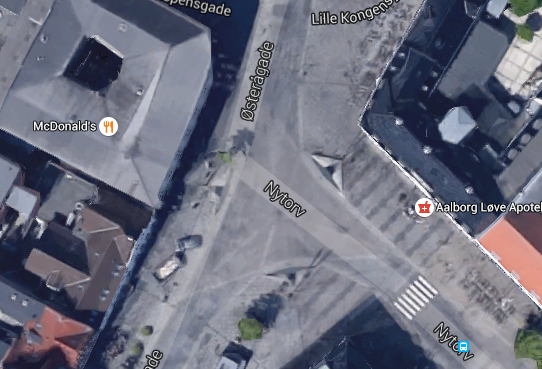
\includegraphics{figures/Billederogfigur/rundkorselplace.png} %googlemaps
  \end{adjustbox}
   \caption{Placering af Rundkørsel}
    \label{fig:rundkorselplace}
 \end{figure}
 \newpage

%rundkorselplace.png
\subsubsection{Fordel og Ulempe}
\label{subs:fordel_og_ulempe}
En fordel ved rundkørsel ved Nytorv området vil være, at alle trafikanter kan færdes uden fare for konflikter, eftersom farten vil bliver sænket drastisk forhold til hvad den er allerede. Derudover vil der blive skabt mere tryghed og sikkerhed for fodgængere, da farten ved området bliver sænket. Eftersom rundkørsel har sine fordele, så har den lige så vel ulemper. Den største ulempe vil nok være, at der mange busser der færdes ved området og skarpe sving er dog ikke det optimale for busser, så det vil skabe forsinkelser i og med, at flere trafikanter skal færdes i et område. En anden ulempe er nok, det kan blive farligt for cyklister, da der er personbiler som krydser Nytorv illegal og ifølge artiklen “Rundkørsler og trafiksikkerhed”, så vil personbiler blive farligt for cyklister ved en rundkørsel.

\subsubsection{Løsning eller ej?}
\label{subs:Losning}

Som umiddelbart vil rundkørsel lyde til, at være en fantastisk ide, eftersom det kan sænke alle mulige uheld med 47 procent. Der kan så antages, at det nok også vil sænke faren for alvorlige konflikter ved området Nytorv. Ifølge observationen, så var der 13 ud af 20 konflikter som var alvorlige, hvis dette kan sænkes med 47 procent, så vil det svar til ca. 6 ud af 20 konflikter vil blive mindre alvorlig. Dog har løsningsforslaget sine ulemper, som kan gøre Nytorv et meget stresset sted for alle trafikantgrupper. Derudover vil det også gå ud over butikker der er  ved området eftersom der kan opstå nogle lange køer ved området.
